\documentclass[conference]{IEEEtran}
\IEEEoverridecommandlockouts
% The preceding line is only needed to identify funding in the first footnote. If that is unneeded, please comment it out.
\usepackage{cite}
\usepackage{amsmath,amssymb,amsfonts}
\usepackage{algorithmic}
\usepackage{graphicx}
\usepackage{textcomp}
\usepackage{xcolor}
\usepackage[brazilian]{babel}
\usepackage[utf8]{inputenc}
\usepackage[T1]{fontenc}
\usepackage{listings}
\usepackage{color}
\usepackage{float}
\usepackage{multirow}

\definecolor{dkgreen}{rgb}{0,0.6,0}
\definecolor{gray}{rgb}{0.5,0.5,0.5}
\definecolor{mauve}{rgb}{0.58,0,0.82}

\lstset{frame=tb,
  language=Java,
  aboveskip=3mm,
  belowskip=3mm,
  showstringspaces=false,
  columns=flexible,
  basicstyle={\small\ttfamily},
  numbers=none,
  numberstyle=\tiny\color{gray},
  keywordstyle=\color{blue},
  commentstyle=\color{dkgreen},
  stringstyle=\color{mauve},
  breaklines=true,
  breakatwhitespace=true,
  tabsize=3
}
\lstset{language=Python}
\def\BibTeX{{\rm B\kern-.05em{\sc i\kern-.025em b}\kern-.08em
    T\kern-.1667em\lower.7ex\hbox{E}\kern-.125emX}}
\begin{document}

\title{Relatório do Laboratório 5: \\ Estratégias Evolutivas\\
}

\author{\IEEEauthorblockN{Isabelle Ferreira de Oliveira}
\IEEEauthorblockA{\textit{CT-213 - Engenharia da Computação 2020} \\
\textit{Instituto Tecnológico de Aeronáutica (ITA)}\\
São José dos Campos, Brasil \\
isabelle.ferreira3000@gmail.com}
}

\maketitle

\begin{abstract}
Esse relatório documenta a implementação de uma estratégia evolutiva simples e comparação de seu desempenho com o de CMA-ES em funções usadas como \textit{benchmark} para algoritmos de otimização. Essas funções utilizadas eram uma esfera transladada, e as fuções de Ackley, Schaffer 2 e Rastrigin 2D.
\end{abstract}

\begin{IEEEkeywords}
Estratégias evolutivas, CMA-ES, \textit{benchmark}, Ackley, Schaffer 2, Rastrigin 2D
\end{IEEEkeywords}

\section{Introdução}
Otimização consiste em encontrar o mínimo (ou máximo) de uma função, ou seja, encontrar o conjunto de parâmetros que levem essa função ao seu mínimo (ou máximo). Também pode ser visto como encontrar a melhor solução dentre todas as soluções viáveis. Nesses problemas de otimização também é possível haver restrições acerca dos parâmetros que serão analisados.

Dentre os mais diversos tipos de algoritmos de otimização, existem os métodos baseado em estratégias evolutivas, métodos esses inspirados na evolução natural das espécies. Esses métodos seguem a ideia de: dada uma população de possíveis soluções, aplica-se uma função para medir a qualidade dessas soluções candidatas. Essa qualidade quantitativa é chamade de \textit{fitness}. Com base no \textit{fitness}, é possível escolher as melhores soluções e, a partir delas, gerar mutações para se criar uma nova população. Esse processo é repetido até que a convergência chegue a um resultado satisfatório de otimização.

O pseudo-código geral de algortimos utilizando estratégias evolutivas pode ser visto a seguir. Em seguida, será apresentado como esse algoritmo foi implementado no contexto do laboratório.

\begin{lstlisting}
def evolution_strategy(J, m0, C0, hyperparams):
	mu, lambda = unwrap_hyperparams(hyperparams)
	m, C = m0, C0
	while not check_stopping_condition():
		population = multivariate_normal(m, C, lambda)
		population = sort_ascending(population, J)
		parents = population[0:mu]
		m = mean(parents)
	return population[0]
\end{lstlisting}

No pseudocódigo acima, \textit{J} é a função para medir a qualidade das soluções candidatas; \textit{m0} e \textit{C0} são a média e a matriz de covariância iniciais da população que será gerada, respectivamente; \textit{m} e \textit{C} são, de forma análoga, a média e a matriz de covariância atuais da população que será gerada, respectivamente; e \textit{mu} é o tamanho da população considerada como "melhores soluções até então".

\section{Implementação do algoritmo}
Na parte relativa a implementação do algoritmo utilizando uma simples estratégia evolutiva (SES, do inglês \textit{Simple Evolution Strategy}), era necessário preencher a função \textit{tell()} da classe \textit{SimpleEvolutionStrategy}. Recebendo os valores de \textit{fitness} encontrados na população anterior, essa função era a responsável por atualizar a média e a matriz de covariância utilizando os melhores avaliados na antiga população e também evoluir a própria população a cada iteração. Essa função a se completar estava no código base fornecido \cite{b1}.  Além disso, era necessário comparar os desempenhos desse algoritmo SES com o algoritmo CMA-ES, já fornecido no código base, aplicando na otimização de quatro funções, a se saber: esfera transladada, e as fuções de Ackley, Schaffer 2 e Rastrigin 2D.

A análise de vários pontos dos algoritmos descritos acima terão uma breve descrição em alto nível da sua implementação a seguir. 

Primeiramente, foi criada uma lista de particulas para a classe principal \textit{ParticleSwarmOptimization}, um contador referente a qual partícula dessa lista o código estará se referindo em uma determinada iteração, além de variáveis para guardar o melhor valor (referente a função qualidade a ser otimizada) encontrado até aquela iteração dentre todas as partículas e qual a posição desse melhor valor.

Essa lista de partículas é formada por objetos da classe \textit{Particle}, e cada partícula contém sua posição, sua velocidade, além da melhor posição referente ao valor calculado da função de qualidade e qual esse melhor valor alcançado pela partícula. A posição e a velocidade inicial de cada partícula é escolhida uniformemente aleatória, respeitando os limites estabelecidos por quem chama o construtor dessa classe. 

As funções \textit{get\underline{\space}best\underline{\space}position()} e \textit{get\underline{\space}best\underline{\space}value()} retornam, respectivamente, a posição referente ao melhor valor encontrado na função qualidade e qual esse melhor valor dentre todas as partidas e todas as iterações. Já a função \textit{get\underline{\space}position\underline{\space}to\underline{\space}evaluate()} se utiliza do contador citado anteriormente para retornar o elemento correto na lista de partículas, ou seja, a próxima partícula a ser analisada.

Por fim, as funções \textit{advance\underline{\space}generation()} e \textit{notify\underline{\space}evaluation()} foram implementadas conforme apresentado nos pseudo códigos da seção Introdução, com alguns detalhes como utilizar o contador referente a qual partícula da lista de partículas o código está se referindo na iteração em questão em \textit{notify\underline{\space}evaluation()}. Além disso, para o caso do robô seguidor de linha, a função \textit{evaluate()} da classe \textit{Simulation} foi implementada conforme o apresentado na Seção 2 do roteiro do laboratório \cite{b1}, com $e_k = 1$ para o caso de não detecção de linha (booleana \textit{detection} sendo \textit{False}) e $\omega = 0.5$. 

\section{Resultados e Conclusões}
A otimização foi executada para duas funções de qualidade: uma função matemática $f\left ( x \right ) = - \left ( x\left ( 0 \right ) - 1 \right )^{2} + \left ( x\left ( 1 \right ) - 2 \right )^{2} + \left ( x\left ( 2 \right ) - 3 \right )^{2}$ e a função \textit{evaluate()} do robô seguidor de linha. Os resultados das otimizações obtidas após a execução da implementação do algoritmo descrito acima foram apresentados nas Figuras de \ref{translated_sphere/ses} a \ref{ackley/cmaes} para a função matemática, e de \ref{line_parameters_convergence} a \ref{line_follower_solution} para o robô seguidor de linha.

\subsection{Função Esfera Transladada}

A partir da Figura \ref{translated_sphere/cmaes}, foi possível notar o correto funcionamento da implementação do algoritmo PSO, uma vez que os parâmetros $x(0)$, $x(1)$ e $x(2)$ convergiram corretamente para os valores 1, 2 e 3, como era esperado. Além disso, as Figuras \ref{ackley/ses} e \ref{ackley/cmaes} comprovaram a convergência da função para $0$, valor máximo também já esperado.

\begin{figure}[htbp]
\centering
\centerline{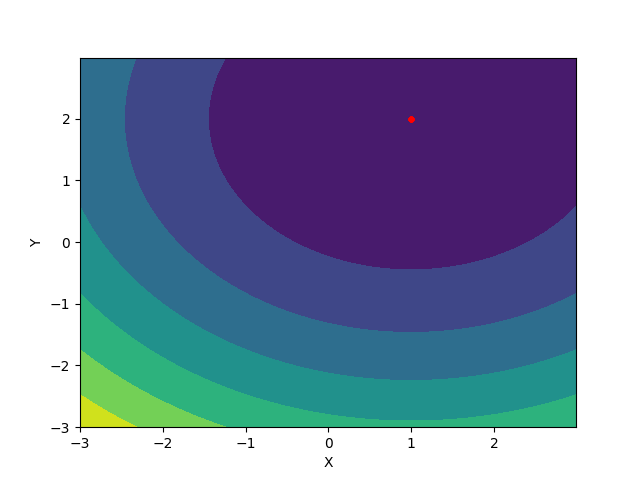
\includegraphics[scale=0.4]{imagens/translated_sphere/ses.png}}
\caption{Valores convergidos dos parâmetros para maximização da função para o caso da função matemática.}
\label{translated_sphere/ses}
\end{figure}

\begin{figure}[htbp]
\centering
\centerline{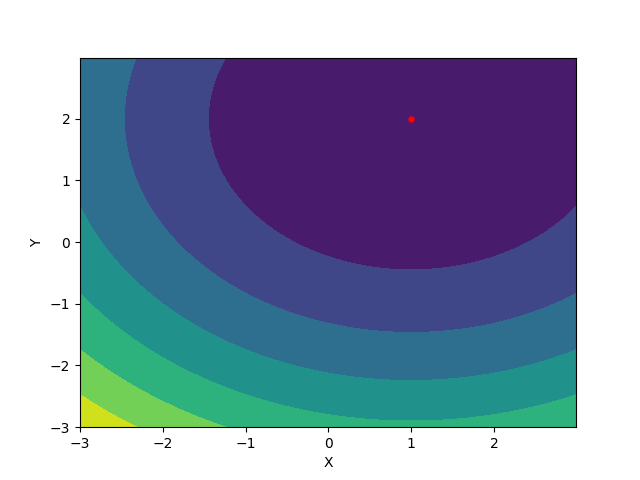
\includegraphics[scale=0.4]{imagens/translated_sphere/cmaes.png}}
\caption{Valores convergidos dos parâmetros para maximização da função para o caso da função matemática.}
\label{translated_sphere/cmaes}
\end{figure}

\begin{figure}[htbp]
\centering
\centerline{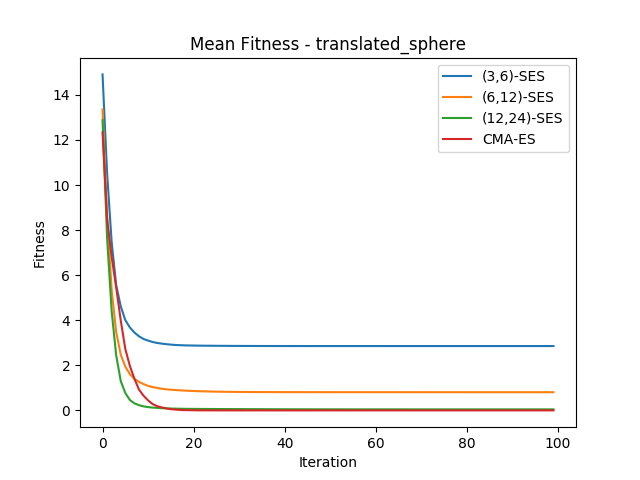
\includegraphics[scale=0.4]{imagens/translated_sphere/mean_fitness.png}}
\caption{Valores convergidos dos parâmetros para maximização da função para o caso da função matemática.}
\label{translated_sphere/mean_fitness}
\end{figure}

\begin{figure}[htbp]
\centering
\centerline{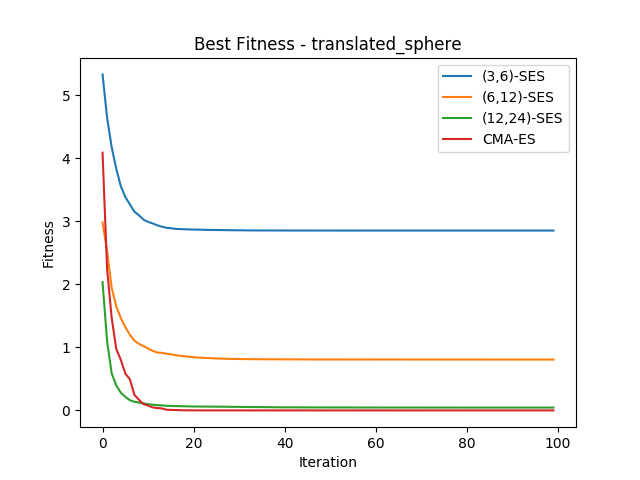
\includegraphics[scale=0.4]{imagens/translated_sphere/best_fitness.png}}
\caption{Valores convergidos dos parâmetros para maximização da função para o caso da função matemática.}
\label{translated_sphere/best_fitness}
\end{figure}

\subsection{Função Ackley}

\begin{figure}[htbp]
\centering
\centerline{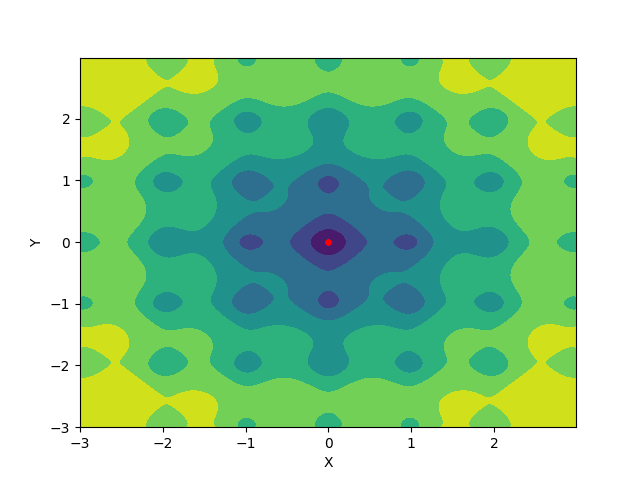
\includegraphics[scale=0.4]{imagens/ackley/ses.png}}
\caption{Convergência do valor da função qualidade com o passar das iterações para o caso da função matemática.}
\label{ackley/ses}
\end{figure} 

\begin{figure}[htbp]
\centering
\centerline{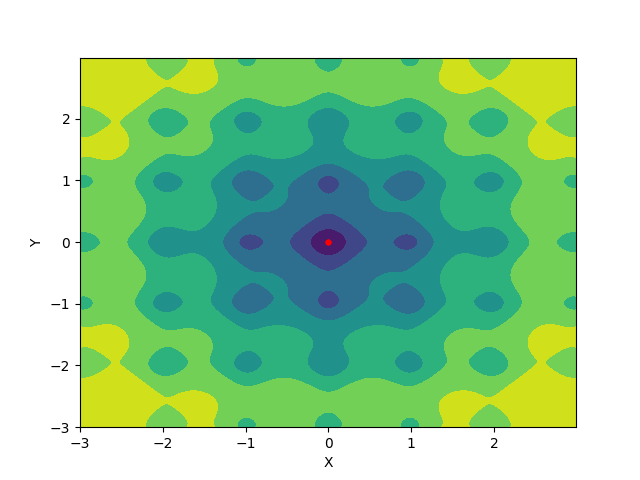
\includegraphics[scale=0.4]{imagens/ackley/cmaes.png}}
\caption{Convergência do melhor valor da função qualidade encontrado com o passar das iterações para o caso da função matemática.}
\label{ackley/cmaes}
\end{figure}

\begin{figure}[htbp]
\centering
\centerline{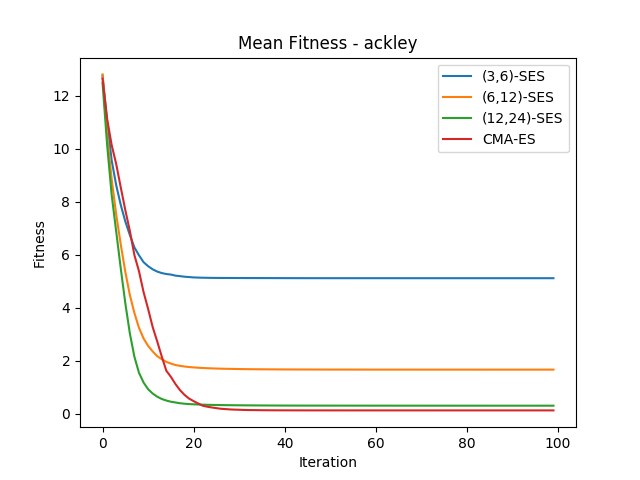
\includegraphics[scale=0.4]{imagens/ackley/mean_fitness.png}}
\caption{Valores convergidos dos parâmetros para maximização da função para o caso da função matemática.}
\label{ackley/mean_fitness}
\end{figure}

\begin{figure}[htbp]
\centering
\centerline{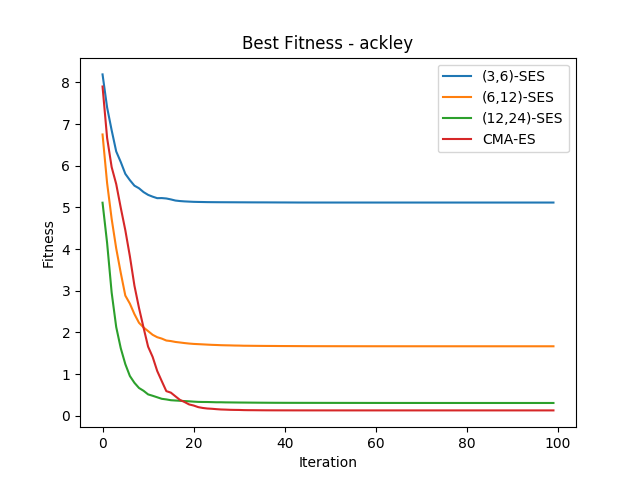
\includegraphics[scale=0.4]{imagens/ackley/best_fitness.png}}
\caption{Valores convergidos dos parâmetros para maximização da função para o caso da função matemática.}
\label{ackley/best_fitness}
\end{figure}

\subsection{Função Schaffer Nº 2}

\begin{figure}[htbp]
\centering
\centerline{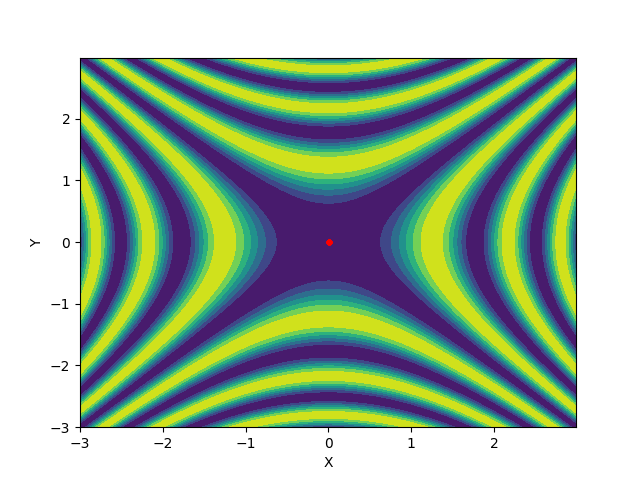
\includegraphics[scale=0.4]{imagens/schaffer2d/ses.png}}
\caption{Convergência do valor da função qualidade com o passar das iterações para o caso da função matemática.}
\label{schaffer2d/ses}
\end{figure} 

\begin{figure}[htbp]
\centering
\centerline{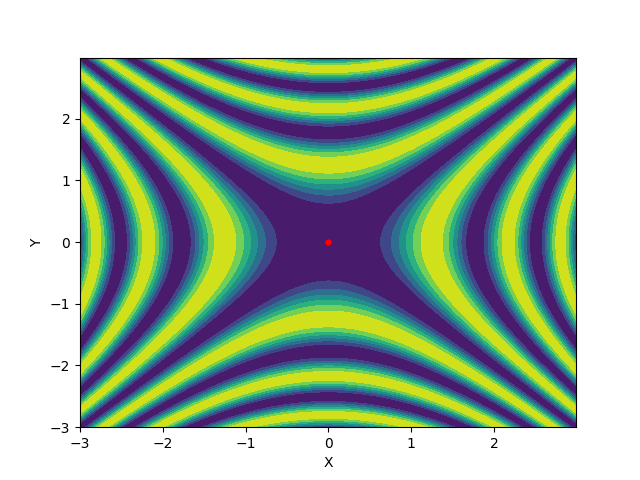
\includegraphics[scale=0.4]{imagens/schaffer2d/cmaes.png}}
\caption{Convergência do melhor valor da função qualidade encontrado com o passar das iterações para o caso da função matemática.}
\label{schaffer2d/cmaes}
\end{figure}

\begin{figure}[htbp]
\centering
\centerline{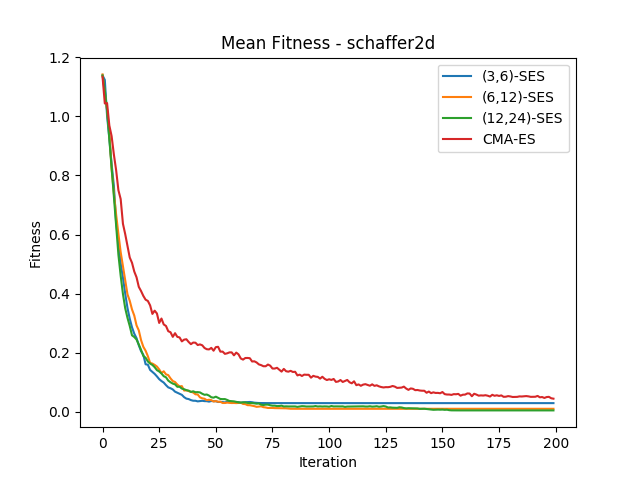
\includegraphics[scale=0.4]{imagens/schaffer2d/mean_fitness.png}}
\caption{Valores convergidos dos parâmetros para maximização da função para o caso da função matemática.}
\label{schaffer2d/mean_fitness}
\end{figure}

\begin{figure}[htbp]
\centering
\centerline{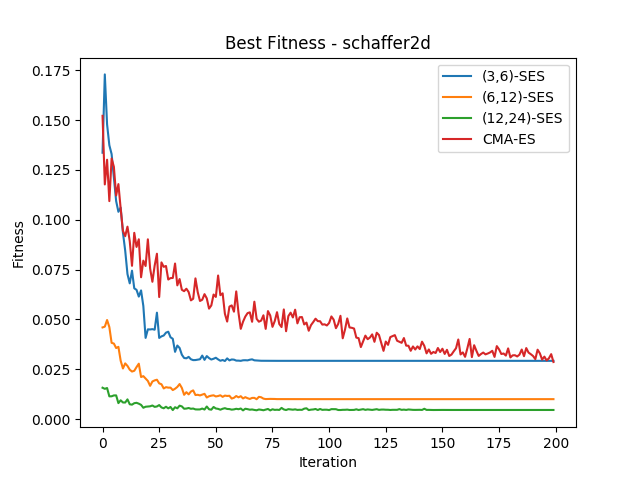
\includegraphics[scale=0.4]{imagens/schaffer2d/best_fitness.png}}
\caption{Valores convergidos dos parâmetros para maximização da função para o caso da função matemática.}
\label{schaffer2d/best_fitness}
\end{figure}

\subsection{Função Rastrigin (2D)}

\begin{figure}[htbp]
\centering
\centerline{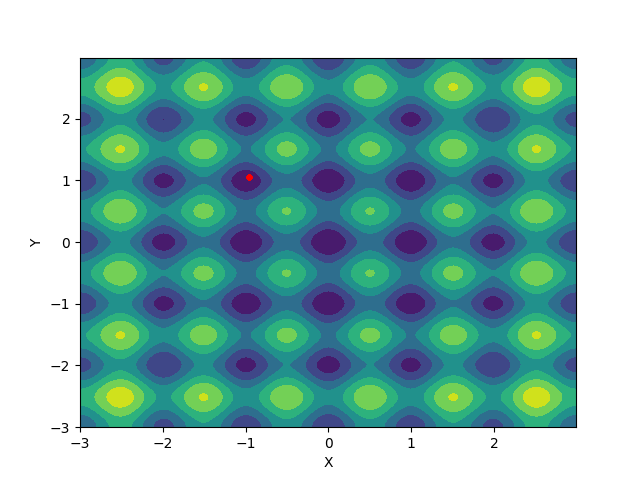
\includegraphics[scale=0.4]{imagens/rastrigin/ses.png}}
\caption{Convergência do valor da função qualidade com o passar das iterações para o caso da função matemática.}
\label{rastrigin/ses}
\end{figure} 

\begin{figure}[htbp]
\centering
\centerline{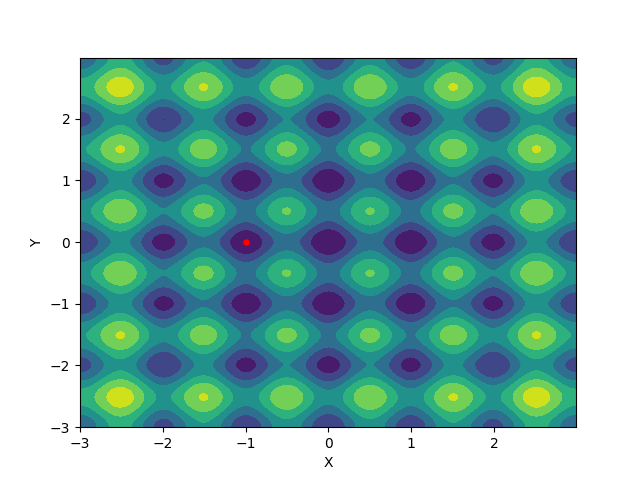
\includegraphics[scale=0.4]{imagens/rastrigin/cmaes.png}}
\caption{Convergência do melhor valor da função qualidade encontrado com o passar das iterações para o caso da função matemática.}
\label{rastrigin/cmaes}
\end{figure}

\begin{figure}[htbp]
\centering
\centerline{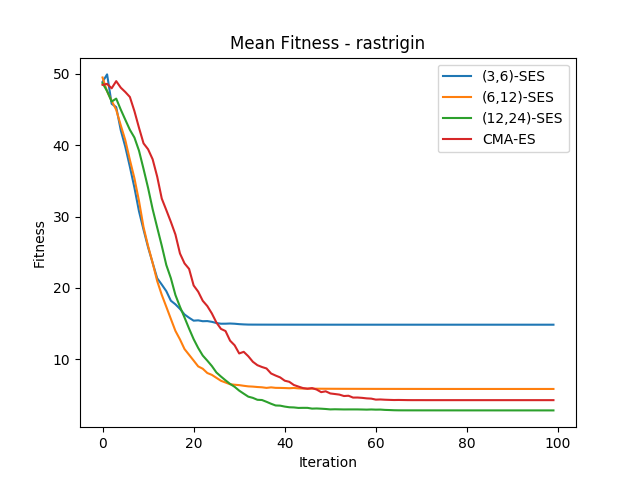
\includegraphics[scale=0.4]{imagens/rastrigin/mean_fitness.png}}
\caption{Valores convergidos dos parâmetros para maximização da função para o caso da função matemática.}
\label{rastrigin/mean_fitness}
\end{figure}

\begin{figure}[htbp]
\centering
\centerline{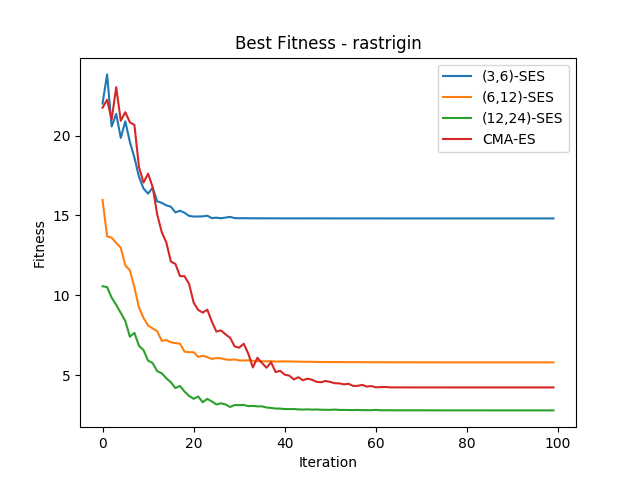
\includegraphics[scale=0.4]{imagens/rastrigin/best_fitness.png}}
\caption{Valores convergidos dos parâmetros para maximização da função para o caso da função matemática.}
\label{rastrigin/best_fitness}
\end{figure}

Tendo em vista o correto funcionamento do algoritmo PSO dado o apresentado na subseção anterior e o comportamento coerente realizado pelo robô apresentado na Figura \ref{line_follower_solution}, pode-se concluir que os resultados apresentados na Figura \ref{line_parameters_convergence} são parâmetros satisfatórios do problema, chegando a convergência maximizada da Figura \ref{line_best_convergence}. Esses valores de parâmetros foram encontrados após cerca de 3000 iterações, levando a um valor de função qualidade máximo de 572.33; parâmetros esses: a velocidade linear do robô (0.72) e os ganhos proporcional, integrativo e derivativo (131.73, 624.82, 15.37, respectivamente).

Tendo em vista o que foi apresentado, pode-se notar, por fim, que esse algoritmo realmente se demonstrou eficaz em encontrar parâmetros otimizados para uma determinada função de custo e um conjunto de possíveis soluções iniciais.

\begin{thebibliography}{00}
\bibitem{b1} M. Maximo, ``Roteiro: Laboratório 4 - Otimização com Métodos Baseados em População''. Instituto Tecnológico de Aeronáutica, Departamento de Computação. CT-213, 2019.
\end{thebibliography}

\end{document}
